\documentclass{beamer}

\usepackage[utf8]{inputenc}
\usetheme{Madrid}
\usepackage[short]{optidef}
\usepackage{caption}
\captionsetup{font=scriptsize,labelfont=scriptsize}
\usepackage{listings}
\usepackage{multimedia}
\graphicspath{{images/}}
\setbeamertemplate{footline}
{
  \leavevmode%
  \hbox{%
  \begin{beamercolorbox}[wd=.4\paperwidth,ht=2.25ex,dp=1ex,center]{author in head/foot}%
    \usebeamerfont{author in head/foot}\insertshortauthor
  \end{beamercolorbox}%
  \begin{beamercolorbox}[wd=.6\paperwidth,ht=2.25ex,dp=1ex,center]{title in head/foot}%
    %\usebeamerfont{title in head/foot}\insertshorttitle\hspace*{3em}
    \insertframenumber{} / \inserttotalframenumber\hspace*{1ex}
  \end{beamercolorbox}}%
  \vskip0pt%
}

\lstset{
numbers = left, 
numberstyle = \tiny, 
numbersep = 8pt, 
frame = single, 
language = Python, 
framexleftmargin = 15pt,
basicstyle=\tiny,
showstringspaces=false}


%Information to be included in the title page:
\title{Sensitivity-Based Economic NMPC with a Path-Following Approach in Python}
\author{Brittany Hall}
\institute{Norwegian University of Science and Technology (NTNU)}
\date{01.11.2017}
\titlegraphic{\includegraphics[height=1.2cm]{ntnu.png}}

\begin{document}

\frame{\titlepage}

%SLIDE 
\begin{frame}{Simple Example Problem}
\begin{columns}
\begin{column}{0.5\textwidth}
	\begin{mini*}
		{x\in\mathbb{R}^2}{p_1x_1^3+x_2^2}{}{}
		\addConstraint{x_2-e^{-x_1}\geq0}{}{}
		\addConstraint{x_1\geq p_2}{}{}
	\end{mini*}
	Use approximate solution $x_0 = (0.5,0.6)$ with $p_0=(1,-4)$ to trace a path to find an approximate solution for $p_f=(8,1)$.
\end{column}
\begin{column}{0.5\textwidth}
	\centering
	\movie[label=false,width=1\textwidth,poster,open,showcontrols]{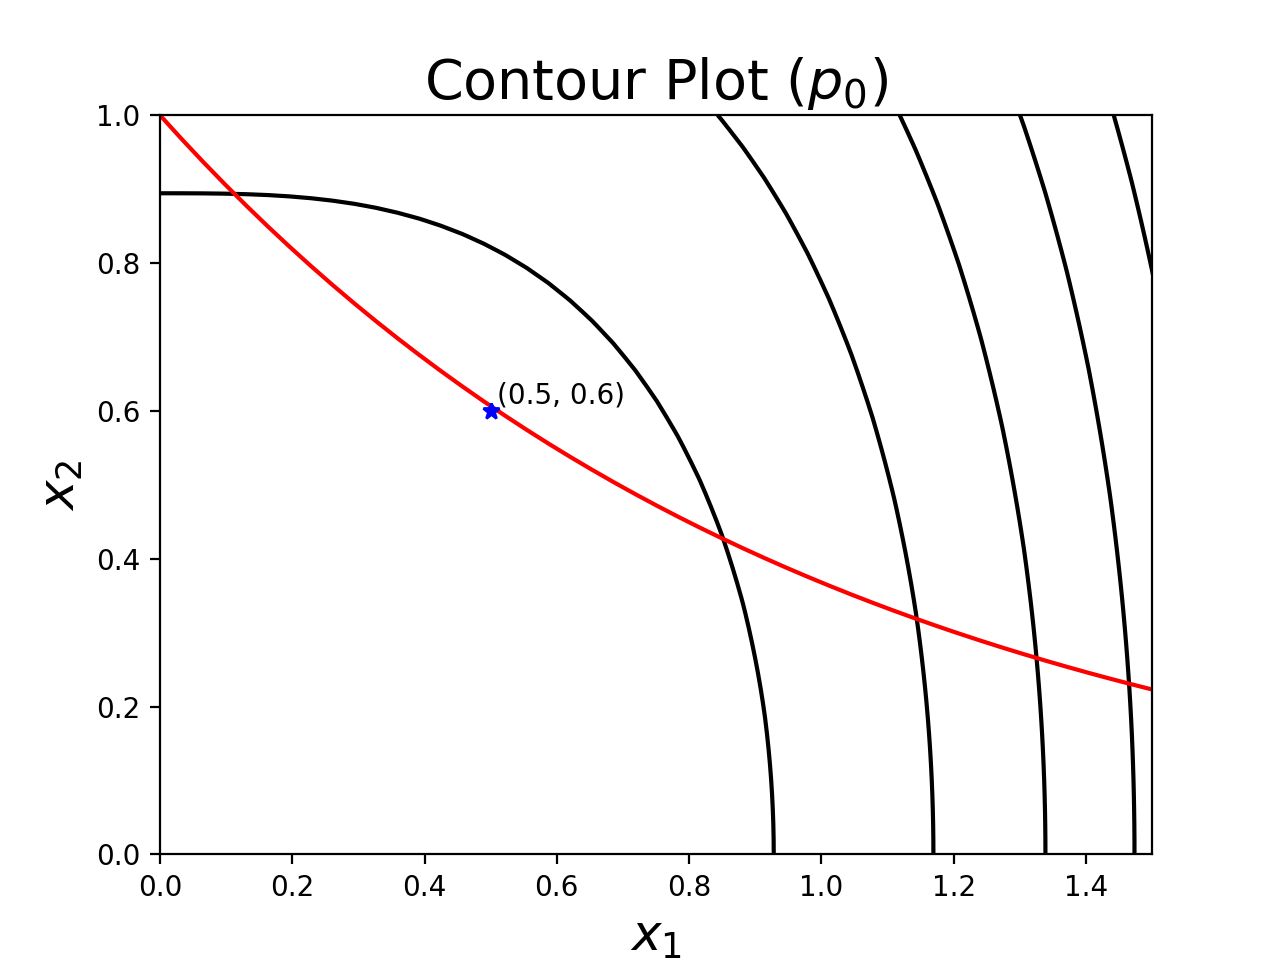
\includegraphics[width=\textwidth]{contour_p0.png}}{contour_plots.avi}
\end{column}
\end{columns}
\end{frame}
%SLIDE
\begin{frame}{CSTR + Distillation Column System}
	\begin{columns}
		\begin{column}{0.5\textwidth}
			\begin{figure}[H]
				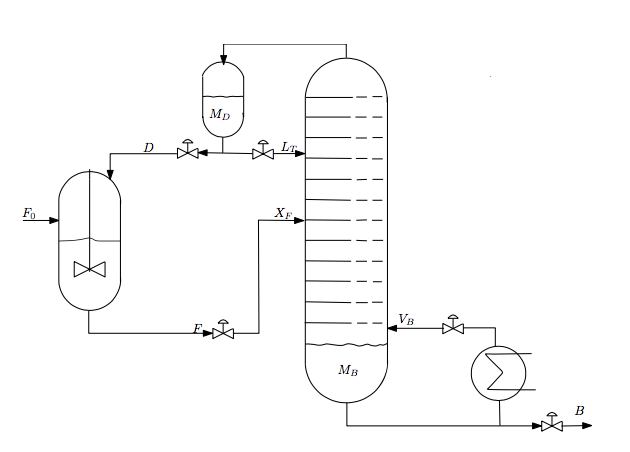
\includegraphics[scale=0.6]{process}
				\caption{CSTR + Distillation column}
			\end{figure}
		\end{column}
		\begin{column}{0.5\textwidth}
			\begin{figure}[H]
				\centering
				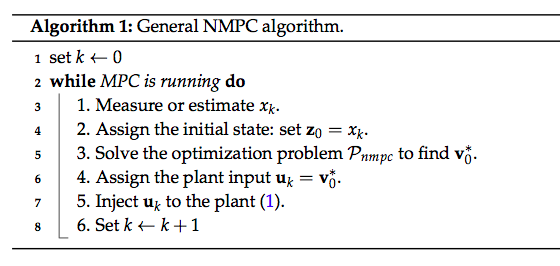
\includegraphics[scale=0.3]{NMPC}
			\end{figure}
			
		\end{column}
	\end{columns}
\end{frame}
%SLIDE
\begin{frame}
Back Up Slides
\end{frame}
%SLIDE
\begin{frame}{Path-following algorithm}
	\begin{figure}[H]
		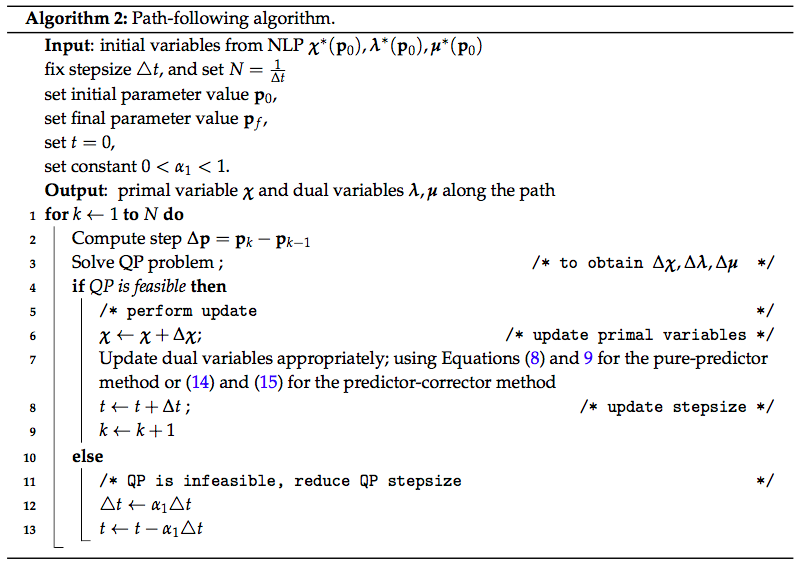
\includegraphics[scale=0.35]{pf_algo}
	\end{figure}
\end{frame}
\end{document}